% !TeX spellcheck = de_DE
\documentclass[.../Dokumentation.tex]{subfiles}
\begin{document}
\subsection{Hard- und Software}
\label{sec-ita1-hardware}

\subsubsection*{Fahrzeug}
Nachdem die Hardware eingetroffen ist, soll in einem ersten Schritt 
die Funktionalität des Hall-Sensors testweise implementiert werden. Das Ziel 
ist herauszufinden, bis zu welchem Abstand der Sensor die Magneten erkennt und 
ob der Einsatz von mehreren Magneten in den Reifen möglich ist. Für den Sensor 
steht nur Dokumentation im Rahmen eines Datenblattes zur Verfügung. Hierbei erweist es sich als schwierig, die Bedeutung der drei Pins zu 
erkennen. Letztendlich stellt sich heraus, dass der linke Pin $+$, der 
mittlere \textit{GND} und der rechte das $Output$ Signal ist.\\
Beim Erstellen der Schaltung entsteht ein weiteres Problem. Der Sensor benötigt für den Betrieb mindestens $3.7V$. Somit muss der $+$-Pin an den $5V$ Pin des 
Arduinos angeschlossen werden. Der $Output$-Pin liefert dementsprechend auch $5V$ muss mit einem IO-Pin des Arduinos verbunden werden, damit das 
Signal von diesem eingelesen werden kann. Laut Datenblatt dürfen an die Pins maximal $3.3V$ angelegt werden, ansonsten droht eine Beschädigung des Arduinos.
\begin{figure}[H]
\begin{center}
    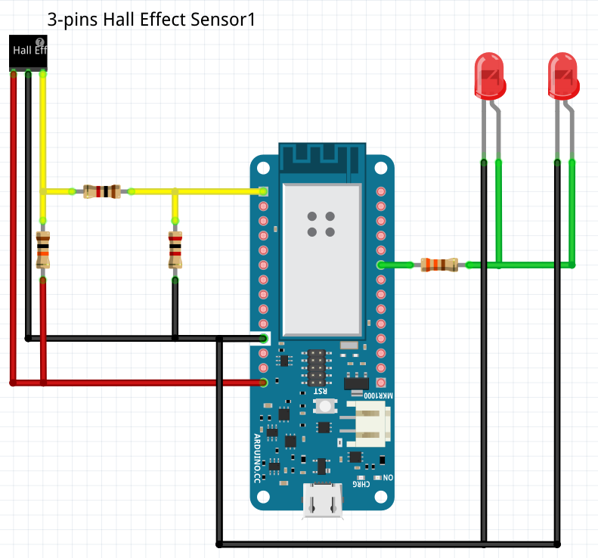
\includegraphics[
    width=0.5\linewidth,
    ]{imgs/hardware_car_iteration1.png}
    \caption{Erstes Konzept des Schaltplans für die Fahrzeuge}
    \label{fig-hardware-car-iteration1}
\end{center}
\end{figure}
\noindent
Mit einem Spannungsteiler, bestehend aus einem $1k\ \Omega$ und einem $2k\ \Omega$ Widerstand, können $5V$ 
auf $3.3V$ runter-gesetzt werden. Zusätzlich soll ein 
$10k\ \Omega$ Pull-Up Widerstand verwendet werden, welcher den verwendeten Pin 
des Arduinos auf \textit{HIGH} setzt, solange kein Magnet erkannt ist. Die verwendete Schaltung ist in Abbildung \ref{fig-hardware-car-iteration1} dargestellt. 
Hierbei werden zusätzlich zwei LEDs hinzugefügt, welche später als Scheinwerfer im Fahrzeug verwendet werden. 
\end{document}